% !TeX program = pdflatex
% Отчёт по заданию 1 «Деградация подшипника» (вариант 13), ГОСТ 7.32-2017.
% Все числа вставляются макросами из tables/macros.tex (см. src/modeling.py):
% ручное редактирование чисел в тексте не требуется и не используется.
\documentclass[14pt,a4paper]{extarticle}

\usepackage[T2A]{fontenc}
\usepackage[utf8]{inputenc}
\usepackage[russian]{babel}
\usepackage{tempora}                % Times-подобный текстовый шрифт
\usepackage{amsmath}
\usepackage{graphicx}
\usepackage{booktabs}
\usepackage{array}
\usepackage{float}
\usepackage{setspace}
\usepackage[a4paper,top=20mm,bottom=20mm,left=30mm,right=15mm]{geometry}
\usepackage{caption}
\usepackage{titlesec}
\usepackage{lastpage}
\usepackage[unicode,hidelinks]{hyperref}

% --- Оформление по ГОСТ 7.32-2017 -----------------------------------------
\onehalfspacing
\setlength{\parindent}{12.5mm}
\setlength{\parskip}{0pt}
\setlength{\emergencystretch}{2em}
\setcounter{tocdepth}{2}

% «Рисунок N --- Название» под рисунком, «Таблица N --- Название» над таблицей
\DeclareCaptionLabelSeparator{gostdash}{ --- }
\captionsetup[table]{labelsep=gostdash,justification=raggedright,
  singlelinecheck=false,position=above,skip=6pt}
\captionsetup[figure]{labelsep=gostdash,justification=centering,
  singlelinecheck=false,position=below,skip=6pt}
\addto\captionsrussian{%
  \renewcommand{\figurename}{Рисунок}%
  \renewcommand{\tablename}{Таблица}%
}

% Заголовки разделов: с абзацного отступа, полужирные
\titleformat{\section}{\bfseries}{\thesection}{0.6em}{}
\titleformat{\subsection}{\bfseries}{\thesubsection}{0.6em}{}
\titlespacing*{\section}{\parindent}{14pt}{10pt}
\titlespacing*{\subsection}{\parindent}{12pt}{8pt}

% Список источников: «1.» в перечне, без собственного заголовка
% (заголовок даёт команда \struct)
\makeatletter
\renewcommand{\@biblabel}[1]{#1.}
\renewenvironment{thebibliography}[1]
     {\list{\@biblabel{\@arabic\c@enumiv}}%
           {\settowidth\labelwidth{\@biblabel{#1}}%
            \leftmargin\labelwidth
            \advance\leftmargin\labelsep
            \usecounter{enumiv}%
            \let\p@enumiv\@empty
            \renewcommand\theenumiv{\@arabic\c@enumiv}}%
      \sloppy
      \clubpenalty\@clubpenalty
      \widowpenalty4000%
      \sfcode`\.\@m}
     {\def\@noitemerr
       {\@latex@warning{Empty `thebibliography' environment}}%
      \endlist}
\makeatother
\addto\captionsrussian{%
  \renewcommand{\refname}{СПИСОК ИСПОЛЬЗОВАННЫХ ИСТОЧНИКОВ}%
}

% Содержание: заголовок по центру, список без полуторного интервала
\makeatletter
\renewcommand\tableofcontents{%
  \clearpage
  \begin{spacing}{1.0}%
  \begin{center}\bfseries СОДЕРЖАНИЕ\end{center}%
  \@starttoc{toc}%
  \end{spacing}%
}
\makeatother

% Структурный элемент: с нового листа, прописными, по центру
\newcommand{\struct}[1]{%
  \clearpage
  \begin{center}\bfseries #1\end{center}%
  \addcontentsline{toc}{section}{#1}%
}

\newcommand{\BestModelName}{Лассо-регрессия, цель min(RUL, C) (худший подшипник (9))}
\newcommand{\BestHyper}{$C$=250, $\alpha$=3,162}
\newcommand{\BestNFeat}{9}
\newcommand{\BestDof}{6}
\newcommand{\BestThrOneSE}{140,8}
\newcommand{\BestMAECV}{101,6}
\newcommand{\BestMAECVstd}{76,9}
\newcommand{\BestRMSECV}{111,5}
\newcommand{\BestRtwoCV}{\textminus{}8,37}
\newcommand{\BestMAETest}{25,9}
\newcommand{\BestRMSETest}{34,6}
\newcommand{\BestRtwoTest}{0,47}
\newcommand{\BestMAETrain}{150,0}
\newcommand{\BestRMSETrain}{232,4}
\newcommand{\BestRtwoTrain}{0,02}
\newcommand{\BestRhoTest}{0,78}
\newcommand{\BaseMAETest}{163,5}
\newcommand{\BaseRMSETest}{170,2}
\newcommand{\OlsMAETest}{3648,1}
\newcommand{\OlsMAECV}{287,2}
\newcommand{\OlsMAETrain}{41,9}
\newcommand{\OlsRtwoTrain}{0,95}
\newcommand{\OlsMinPred}{\textminus{}7723}
\newcommand{\PhysAMAETest}{1724,2}
\newcommand{\PhysBMAETest}{65,0}
\newcommand{\RidgeAMAETest}{80,8}
\newcommand{\LassoAMAETest}{164,0}
\newcommand{\OlsBMAETest}{996,4}
\newcommand{\RidgePolyBMAETest}{448,4}
\newcommand{\RidgeBMAETest}{40,9}
\newcommand{\ENetBMAETest}{32,7}
\newcommand{\ENetAMAETest}{81,2}
\newcommand{\RhoResidPred}{0,29}
\newcommand{\RhoResidRMS}{\textminus{}0,31}
\newcommand{\RhoResidKurt}{0,11}
\newcommand{\NTrain}{2156}
\newcommand{\NHoldout}{984}
\newcommand{\DurTrain}{828}
\newcommand{\DurHoldout}{164}
\newcommand{\RulMaxTrain}{828}
\newcommand{\RulMaxHoldout}{164}

\begin{document}

% ============================================================================
% Титульный лист
% ============================================================================
\begin{titlepage}
\begin{center}
{\normalsize МИНИСТЕРСТВО НАУКИ И ВЫСШЕГО ОБРАЗОВАНИЯ\\ РОССИЙСКОЙ ФЕДЕРАЦИИ}\\[3mm]
{\normalsize ФЕДЕРАЛЬНОЕ ГОСУДАРСТВЕННОЕ БЮДЖЕТНОЕ ОБРАЗОВАТЕЛЬНОЕ\\
УЧРЕЖДЕНИЕ ВЫСШЕГО ОБРАЗОВАНИЯ}\\[1mm]
{\normalsize «САНКТ-ПЕТЕРБУРГСКИЙ ГОСУДАРСТВЕННЫЙ УНИВЕРСИТЕТ»}\\[20mm]

{\normalsize Кафедра гидроаэромеханики}\\[24mm]

{\large ОТЧЁТ}\\[4mm]
{\normalsize по дисциплине «Машинное обучение»}\\[4mm]
{\normalsize на тему: «Задание 1. Линейные модели.\\ Деградация подшипника»}\\[2mm]
{\normalsize (вариант 13)}\\[30mm]
\end{center}

\begin{flushright}
\begin{tabular}{l}
Выполнил: студент группы st117207\\[1mm]
\hspace{25mm}Белобородов Д.~А.\\[3mm]
Проверил: \underline{\hspace{45mm}}\\
\end{tabular}
\end{flushright}

\vfill
\begin{center}
{\large Санкт-Петербург}\\[2mm]
{\large 2026}
\end{center}
\end{titlepage}
\setcounter{page}{2}

% ============================================================================
% Реферат
% ============================================================================
\struct{РЕФЕРАТ}

\noindent Отчёт \pageref{LastPage}~с., 8~рис., 6~таб., 9~источн., 2~прил.

\vspace{4mm}
\noindent\textbf{МАШИННОЕ ОБУЧЕНИЕ, ЛИНЕЙНАЯ РЕГРЕССИЯ, ГРЕБНЕВАЯ РЕГРЕССИЯ,
ЛАССО, УПРУГАЯ СЕТЬ, ОСТАТОЧНЫЙ РЕСУРС, ДЕГРАДАЦИЯ ПОДШИПНИКА,
ВИБРОДИАГНОСТИКА, КРОСС-ВАЛИДАЦИЯ, БУТСТРЭП}

\vspace{4mm}
\noindent
В отчёте рассмотрена задача прогноза времени, остающегося до конца стендового
испытания подшипников, по записям виброакселерометров набора NASA IMS.
Цель работы~--- построить линейные модели такого прогноза и проверить,
переносятся ли они на испытание, которое целиком отложено от обучения.

Из каждого сигнала извлечены физически осмысленные характеристики: RMS,
дисперсия, эксцесс, пик-фактор и доли энергии в пяти широких частотных
полосах, с нормировкой амплитудных величин на здоровый базовый уровень
начала испытания. Рассмотрена физически мотивированная постановка, в которой
целью служит усечённое значение $\min(RUL, C)$. Обучены МНК, гребневая,
лассо-регрессия и упругая сеть; гиперпараметры подобраны кросс-валидацией
по временным складкам только на обучающем испытании, отложенный тест
использован один раз.

Лучшей по правилу одного стандартного отклонения оказалась лассо-регрессия
по девяти признакам «худшего подшипника» (\BestHyper, эффективное число
параметров \BestDof). На отложенном испытании её MAE равен \BestMAETest~ч
($R^2=\BestRtwoTest$, ранговая корреляция Спирмена \BestRhoTest), тогда как
у базовой модели~--- \BaseMAETest~ч. Главный вывод работы: интерполяционная
оценка (кросс-валидация) не гарантирует переноса~--- модели, обученные
на отдельных каналах испытания, выигрывают в кросс-валидации, но заметно
теряют на отложенном испытании, потому что отказ произошёл в другом
подшипнике.

% ============================================================================
\tableofcontents

% ============================================================================
\struct{ВВЕДЕНИЕ}

Подшипники качения~--- самый массовый и самый «хрупкий» узел роторных машин:
износ колец и тел качения развивается постепенно, но заканчивается внезапным
заклиниванием. Если научиться по текущей вибрации оценивать, сколько времени
осталось до отказа, обслуживание можно планировать заранее, а не по факту
аварии. Этим объясняется интерес к задаче, которую в англоязычной литературе
называют prognosis (прогнозирование остаточного ресурса).

Набор IMS (Intelligent Maintenance Systems) хорошо подходит для такой
постановки: в нём есть полные записи жизненного цикла подшипников~--- от
здорового состояния до остановки стенда по отказу. Это редкость: обычно
историю деградации приходится восстанавливать по обрывкам данных.

Цель настоящей работы~--- построить линейные модели прогноза времени,
остающегося до конца испытания, по признакам вибрационного сигнала
и проверить их переносимость на испытание, полностью отложенное от обучения.

Работа выполнена в следующем порядке:
\begin{enumerate}
  \item подготовлены данные: набор IMS загружен, распакован, из каждой записи
  извлечены признаки, заданные вариантом 13;
  \item до обучения сформулированы проверяемые гипотезы о связи признаков
  с оставшимся ресурсом;
  \item реализовано только временное разбиение данных; гиперпараметры
  подобраны кросс-валидацией на обучающем испытании;
  \item обучены обязательные линейные модели (МНК, гребневая регрессия,
  лассо, упругая сеть) и базовая модель сравнения;
  \item качество оценено (MAE, RMSE, $R^2$) на обучении, кросс-валидации
  и однократно на отложенном испытании;
  \item устойчивость коэффициентов проверена бутстрэпом, остатки~---
  стандартной диагностикой;
  \item интерполяционная оценка качества сопоставлена с качеством переноса,
  сделаны выводы.
\end{enumerate}

% ============================================================================
\section{ПОСТАНОВКА ЗАДАЧИ И ИСХОДНЫЕ ДАННЫЕ}

\subsection{Формулировка варианта}

Вариант 13 задания 1 формулируется так: по набору данных NASA IMS требуется
предсказывать время, остающееся до конца данного эксперимента. На каждую
запись вычисляются RMS, дисперсия, эксцесс, пик-фактор и энергии в заданных
широких полосах спектра. Номер записи и абсолютное время в качестве признаков
запрещены~--- иначе модель «подсмотрела бы» календарь вместо состояния
подшипника. Разбиение данных допускается только временное, и одно из
испытаний полностью откладывается для финальной проверки. Модели обязаны
быть линейными по коэффициентам; полином второй степени разрешён сразу,
третья~--- только если кросс-валидация подтвердит её полезность.

Величину, которую мы предсказываем, стоит объяснить подробнее. Пусть $t$~---
отметка времени текущей записи (она берётся из имени файла, но только
в целевую переменную, не в признаки). Тогда
\begin{equation}
RUL_t = t_{\text{кон}} - t, \qquad t_{\text{кон}} = \max_j t_j \text{ в данном испытании}.
\label{eq:rul}
\end{equation}
Это прокси-ресурс: настоящее время до отказа нам не известно, испытание
останавливается постфактум, поэтому единственная честная величина, доступная
одновременно для всех записей испытания,~--- оставшаяся длина самого
испытания.

\subsection{Набор данных IMS}

Использованы два испытания набора IMS. Запись длится 1~с при частоте опроса
20~кГц (20480 отсчётов на канал), интервал между записями~--- 10~мин, только
первые 43 записи испытания 1 идут через каждые 5~мин. Каналы~--- это
сигналы акселерометров: виброускорение подшипникового узла, измеряемое
в единицах свободного падения $g$ (примерно $9{,}8~\text{м/с}^2$);
отсюда все входные переменные имеют единицы либо ускорения (RMS,
дисперсия, пик-фактор~--- в $g$ и его производных), либо безразмерные
(эксцесс, доли энергии полос). Целевая величина~--- время, единицы
измерения~--- часы. В испытании 1
восемь каналов~--- четыре подшипника, по два ортогональных акселерометра
на каждый; испытание остановлено при деградации наружного кольца подшипника
№3 и роликов подшипника №4. В испытании 2 четыре канала (по одному
акселерометру на подшипник), остановка по отказу наружного кольца подшипника
№1. Сводка~--- в таблице~\ref{tab:data}.

\begin{table}[H]
\centering
\small
\setlength{\tabcolsep}{5pt}
\caption{Характеристика исходных испытаний}\label{tab:data}
\begin{tabular}{p{3.9cm}p{4.3cm}p{4.3cm}}
\toprule
Параметр & Испытание 1 (обучение) & Испытание 2 (тест) \\
\midrule
Число записей & 2156 & 984 \\
Период & 22.10.2003 --- 25.11.2003 & 12.02.2004 --- 19.02.2004 \\
Длительность, ч & 827,5 & 163,8 \\
Максимум прокси-ресурса, ч & 827,5 & 163,8 \\
Отказавший подшипник & №3 (внутр. кольцо), №4 (ролики) & №1 (наружн. кольцо) \\
\bottomrule
\end{tabular}
\end{table}

Обратим внимание на важную деталь, которая потом окажется в центре всей
работы: отказавшие подшипники в двух испытаниях~--- разные. В обучающем
испытании деградируют подшипники №3 и №4, а подшипник №1, отказавший
в отложенном испытании, остаётся здоровым от начала до конца обучения.
Модель, которая «запомнит» каналы именно третьего и четвёртого подшипников,
на новом испытании окажется не у дел~--- этот риск мы заложили в одну
из гипотез заранее.

\subsection{Гипотезы и исследовательские вопросы}

До обучения моделей сформулированы три гипотезы.

\begin{description}
  \item[H1 (амплитудная).] По мере износа амплитуда вибрации отказавшего
  подшипника (RMS, дисперсия) монотонно растёт. Поэтому относительное
  превышение амплитуды над здоровым базовым уровнем должно быть отрицательно
  связано с оставшимся временем: чем сильнее вырос сигнал, тем ближе конец.
  \item[H2 (спектральная).] Энергия по мере разрушения поверхностей качения
  перетекает из низких частот в высокие (3--10~кГц), где сосредоточены
  характерные составляющие дефектов подшипников. Тогда доли энергии полос
  информативны даже там, где абсолютная амплитуда ещё ни о чём не говорит.
  \item[H3 (переносимость).] Отказ в новом испытании может случиться в любом
  подшипнике. Модель, привязанная к конкретным каналам обучающего испытания,
  перенесётся плохо; агрегат «худший подшипник» (поэлементный максимум
  признаков по подшипникам) по построению отвечает на вопрос «как себя
  чувствует самый изношенный узел» и должен переноситься лучше.
\end{description}

Исследовательские вопросы работы: какие характеристики сигнала меняются
перед концом испытания и переносятся ли выводы, сделанные по обучающему
испытанию, на отложенное.

% ============================================================================
\section{МЕТОДИКА}

\subsection{Признаки}

Для каждой записи (20480 отсчётов на канал) на каждом канале вычисляются:
RMS, дисперсия $\sigma^2$, эксцесс (kurtosis) и пик-фактор
$c_{\text{peak}} = \max|x|/\mathrm{RMS}$, а также доли энергии
$E_i = \sum_{f \in B_i} |X(f)|^2 \big/ \sum_f |X(f)|^2$
в пяти широких полосах $B_i$: 0--1, 1--2, 2--3, 3--5 и 5--10~кГц.

Каналы одного подшипника объединяются в признак записи по подшипнику:
RMS~--- по энергии (квадратам), дисперсия и доли полос~--- средним,
эксцесс и пик-фактор~--- максимумом. Затем амплитудные признаки (RMS,
дисперсия, пик-фактор) нормируются на здоровый базовый уровень~--- медиану
первых 10\,\% записей данного испытания~--- и логарифмируются:
\begin{equation}
x^{\text{отн}} = \lg\!\left(\frac{x}{\operatorname{med}\, x_{\text{баз}}}\right).
\label{eq:logrel}
\end{equation}
Логика такой нормировки проста. Уровень сигнала на стенде зависит от
установки датчиков и от конкретного экземпляра подшипника, поэтому
абсолютные вольты из одного испытания нельзя напрямую сравнивать с другим.
Отношение к собственному «здоровому» уровню это сравнение делает возможным,
а логарифм линеаризует быстрый (почти экспоненциальный) рост амплитуды
в конце жизни. Эксцесс, пик-фактор и доли полос~--- безразмерные величины,
они используются без преобразования.

Так получаются две конфигурации признаков:
конфигурация А «по подшипникам»~--- 36 признаков
($4$ подшипника $\times$ (3 нормированных амплитудных + эксцесс + 5 полос))
и конфигурация Б «худший подшипник»~--- 9 признаков, поэлементный максимум
каждой характеристики по четырём подшипникам. Полный состав признаков
вынесен в приложение Б.

\subsection{Физически мотивированная постановка}

Здесь мы отошли от буквальной формулы \eqref{eq:rul}, и на это есть
физическая причина. Пока подшипник исправен, «время до конца испытания»~---
это просто оставшаяся длительность запланированного стенда: она известна
постфактум, но не содержится в вибрации. Убывать ресурс начинает только
с момента зарождения дефекта, и его величина в исправной зоне ограничена
некоторым порогом. Поэтому вместо сырой цели \eqref{eq:rul} предсказывается
кусочно-линейная величина
\begin{equation}
y = \min(RUL, C),
\label{eq:cap}
\end{equation}
где порог $C$~--- плато исправного состояния~--- подбирается кросс-валидацией
по сетке $C \in \{160, 200, 250, 300\}$~ч. Преобразование цели реализовано
через \texttt{TransformedTargetRegressor}: конвейер обучается на усечённой
цели, а прогноз возвращается в исходном масштабе без обратного
преобразования.

Второе предохранение касается области применимости. Линейная модель не должна
экстраполировать по признакам туда, где у неё не было обучающих примеров:
в новом испытании амплитуда может превысить всё виденное при обучении.
Для этого конвейерный преобразователь \texttt{RangeClipper} запоминает
диапазон каждого признака на обучении и заменяет значения вне $[\min, \max]$
границами~--- модель отвечает «вне моей компетенции» не числом, а константой.
Стандартизация признаков выполняется внутри конвейера и обучается только
на обучающих складках~--- иначе информация с теста просочилась бы
в масштабирование.

\subsection{Разбиение и кросс-валидация}

Единственный используемый вид разбиения~--- временное, как и требует вариант.
Испытание 1 целиком ($\NTrain$ записей) образует обучающую выборку;
испытание 2 целиком ($\NHoldout$ записей)~--- отложенный тест. Тест
участвует в работе ровно один раз, в самом конце,~--- любой подбор
по нему означал бы подгонку под ответ.

Подбор гиперпараметров выполнен решётчатым поиском по сетке
(\texttt{Grid\-Search\-CV})
со скользящей кросс-валидацией \texttt{Time\-Series\-Split(5)} по обучающему
испытанию: складки идут в порядке времени, и в каждой складке проверка
расположена позже обучения~--- будущее не может подсказывать прошлое.
Целевая метрика подбора~--- MAE. Случайные состояния всех генераторов
зафиксированы (\texttt{random\_state}=42).

\subsection{Модели}

Обучаются обязательные линейные модели в обеих конфигурациях признаков,
всего 12 моделей плюс базовая:

\begin{enumerate}
  \item базовая модель~--- константный прогноз медианы обучающей цели;
  \item МНК на сырой цели \eqref{eq:rul}~--- наивная постановка, включённая
  специально, чтобы проверить, действительно ли без физической постановки
  нельзя обойтись;
  \item МНК с целью \eqref{eq:cap}~--- физическая постановка;
  \item гребневая регрессия (Ridge) с полиномиальными признаками степени
  $d \in \{1,2\}$, а для конфигурации Б дополнительно $d=3$; после расширения
  выполняется повторная стандартизация, поскольку квадраты и произведения
  живут в другом масштабе, чем исходные признаки;
  \item гребневая регрессия (Ridge);
  \item лассо-регрессия (Lasso);
  \item упругая сеть (Elastic Net) с $l_1 \in \{0{,}1;\ 0{,}5;\ 0{,}9\}$.
\end{enumerate}

Коэффициент регуляризации $\alpha$ перебирается по логарифмической сетке
из 29 точек от $10^{-3}$ до $10^4$.

Итоговая модель выбирается по правилу одного стандартного отклонения
(1SE)~\cite{hastie}: среди моделей, чей MAE КВ не превышает минимум более чем
на одно стандартное отклонение по складкам, берётся модель с наименьшим
эффективным числом параметров (числом ненулевых коэффициентов); при
равенстве~--- с лучшим MAE КВ. Смысл правила в том, что модели, статистически
неразличимые по кросс-валидации, не обязаны одинаково вести себя на новых
данных, и из них разумно выбрать самую разреженную и устойчивую. Для задачи
с заведомым распределительным сдвигом (другой отказавший подшипник) это
особенно уместно.

\subsection{Метрики и оценка неопределённости}

Качество оценивается MAE, RMSE и $R^2$ на трёх выборках (обучение,
кросс-валидация, отложенный тест), а на тесте ещё и ранговой корреляцией
Спирмена между прогнозом и измеренным ресурсом~--- она показывает, верно
ли модель упорядочивает записи по «близости к концу», даже если масштаб
прогноза смещён.

Неопределённость коэффициентов итоговой модели оценена бутстрэпом~\cite{efron}:
300 ресэмплов обучающей выборки с повторениями, для каждого~--- полное
повторное обучение конвейера; по распределению каждого коэффициента берутся
медиана и 95\,\%-ные процентильные интервалы. Диагностика остатков
на отложенном испытании включает зависимость остатков от прогноза и ключевых
признаков, а также ранговые корреляции остатков с факторами
(табл.~\ref{tab:resid}).

% ============================================================================
\section{РЕЗУЛЬТАТЫ}

\subsection{Разведочный анализ}

Сначала~--- о том, как выглядит сама деградация. На
рисунке~\ref{fig:degradation} показан ход RMS по подшипникам в обоих
испытаниях. В испытании 1 RMS подшипников №3 и №4 за последние часы жизни
вырастает на порядок, тогда как подшипники №1 и №2 остаются на одном уровне
до самой остановки. В испытании 2 картина зеркальная: деградирует только
подшипник №1. То есть отказавший подшипник не совпадает с обучающим
испытанием ни по номеру, ни по каналам~--- это видно глазом ещё до всякого
моделирования.

\begin{figure}[H]
\centering
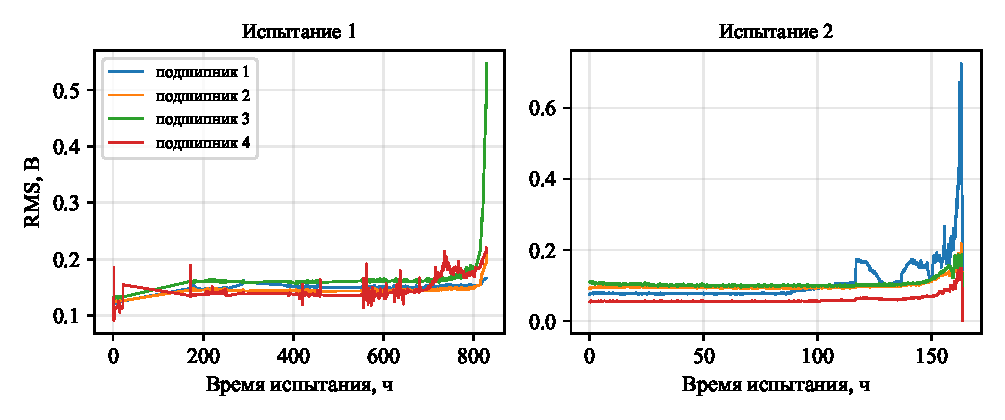
\includegraphics[width=\textwidth]{figures/fig1_degradation.pdf}
\caption{RMS по подшипникам в течение испытаний}
\label{fig:degradation}
\end{figure}

Гипотеза H1 этим подтверждается: в поздней стадии амплитуда растёт в 2--10 раз
относительно базового уровня. Гипотеза H2 подтверждается
рисунком~\ref{fig:bands}: перед концом испытания доля энергии в полосах
3--5 и 5--10~кГц заметно растёт, что соответствует появлению
высокочастотных составляющих от разрушения поверхностей качения. Любопытно,
что в испытании 1 спектральный сдвиг начинается за десятки часов до
остановки, когда RMS ещё не вырос; в испытании 2, которое короче, тот же
сдвиг сжат в последние десятки часов. Доли полос действительно несут
информацию, дополнительную к амплитуде.

\begin{figure}[H]
\centering
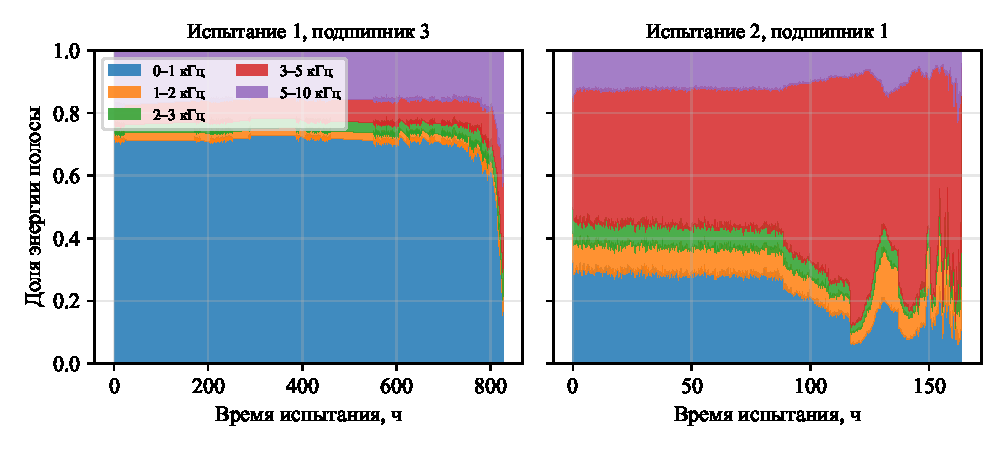
\includegraphics[width=\textwidth]{figures/fig2_bands.pdf}
\caption{Перераспределение энергии по частотным полосам для отказавшего
подшипника}
\label{fig:bands}
\end{figure}

\subsection{Сравнение моделей}

Подобранные гиперпараметры и MAE кросс-валидации всех моделей собраны
в таблице~\ref{tab:hyper}, полные метрики на трёх выборках~--- в
таблице~\ref{tab:metrics}. Кривые валидации (рисунок~\ref{fig:validation})
показывают MAE КВ в зависимости от коэффициента регуляризации и степени
полинома для конфигурации Б: оптимум лежит в области умеренной регуляризации,
а переход к полиному второй степени улучшает MAE КВ; в конфигурации А полином
степени выше первой преимущества не даёт.

\begin{table}[H]
\centering
\small
\setlength{\tabcolsep}{3pt}
\caption{Подобранные по кросс-валидации гиперпараметры моделей}\label{tab:hyper}
\begin{tabular}{>{\raggedright\arraybackslash}p{2.7cm}c>{\raggedright\arraybackslash}p{3.3cm}cc}
\toprule
Модель & Призн. & Гиперпараметры & $p_{\text{эф}}$ & MAE КВ, ч \\
\midrule
Базовая (медиана) & А &  & 1 & 254,4 \\
МНК (наивная) & А &  & 37 & 287,2 \\
МНК + цель min(RUL, C) & А & $C$=250 & 37 & 103,2 \\
Полином + гребень & А & $\alpha$=100,000, $C$=300, $d$=1 & 37 & 81,3 \\
Ridge & А & $\alpha$=100,000, $C$=300 & 37 & 81,3 \\
Lasso & А & $\alpha$=0,316, $C$=300 & 28 & 81,0 \\
Elastic Net & А & $\alpha$=0,056, $C$=300, $l_1$=0.1 & 35 & 81,1 \\
МНК (наивная) & Б &  & 10 & 217,6 \\
МНК + цель min(RUL, C) & Б & $C$=250 & 10 & 104,8 \\
Полином + гребень & Б & $\alpha$=0,056, $C$=250, $d$=2 & 55 & 91,1 \\
Ridge & Б & $\alpha$=316,228, $C$=250 & 10 & 103,3 \\
Lasso & Б & $\alpha$=3,162, $C$=250 & 6 & 101,6 \\
Elastic Net & Б & $\alpha$=0,562, $C$=250, $l_1$=0.9 & 9 & 103,2 \\
\bottomrule
\end{tabular}
\end{table}

\begin{table}[H]
\centering
\caption{Метрики качества моделей: MAE, RMSE, $R^2$ (часы до конца испытания)}\label{tab:metrics}
\resizebox{\textwidth}{!}{%
\begin{tabular}{p{2.9cm}c rrr rrr rrr}
\toprule
 & & \multicolumn{3}{c}{Обучение} & \multicolumn{3}{c}{Кросс-валидация} & \multicolumn{3}{c}{Тест (испытание 2)} \\
\cmidrule(lr){3-5}\cmidrule(lr){6-8}\cmidrule(lr){9-11}
Модель & Призн. & MAE & RMSE & $R^2$ & MAE & RMSE & $R^2$ & MAE & RMSE & $R^2$ \\
\midrule
Базовая (медиана) & А & 192,2 & 246,0 & \textminus{}0,09 & 254,4 & 260,4 & \textminus{}102,10 & 163,5 & 170,2 & \textminus{}11,93 \\
МНК (наивная) & А & 41,9 & 53,8 & 0,95 & 287,2 & 378,3 & \textminus{}607,69 & 3648,1 & 5626,3 & \textminus{}14122,62 \\
МНК + цель min(RUL, C) & А & 139,7 & 225,1 & 0,08 & 103,2 & 122,9 & \textminus{}12,59 & 1724,2 & 1797,9 & \textminus{}1441,21 \\
Полином + гребень & А & 128,8 & 201,1 & 0,27 & 81,3 & 89,4 & \textminus{}4,41 & 80,8 & 135,1 & \textminus{}7,14 \\
Ridge & А & 128,8 & 201,1 & 0,27 & 81,3 & 89,4 & \textminus{}4,41 & 80,8 & 135,1 & \textminus{}7,14 \\
Lasso & А & 126,7 & 199,7 & 0,28 & 81,0 & 89,5 & \textminus{}4,43 & 164,0 & 206,4 & \textminus{}18,01 \\
Elastic Net & А & 129,0 & 201,2 & 0,27 & 81,1 & 89,2 & \textminus{}4,35 & 81,2 & 134,7 & \textminus{}7,09 \\
МНК (наивная) & Б & 100,5 & 123,0 & 0,73 & 217,6 & 245,1 & \textminus{}162,28 & 996,4 & 1021,7 & \textminus{}464,75 \\
МНК + цель min(RUL, C) & Б & 147,8 & 230,7 & 0,04 & 104,8 & 115,9 & \textminus{}10,04 & 65,0 & 74,5 & \textminus{}1,48 \\
Полином + гребень & Б & 140,6 & 226,4 & 0,07 & 91,1 & 104,2 & \textminus{}5,30 & 448,4 & 472,3 & \textminus{}98,51 \\
Ridge & Б & 150,8 & 232,4 & 0,02 & 103,3 & 114,1 & \textminus{}9,18 & 40,9 & 51,2 & \textminus{}0,17 \\
Lasso & Б & 150,0 & 232,4 & 0,02 & 101,6 & 111,5 & \textminus{}8,37 & 25,9 & 34,6 & 0,47 \\
Elastic Net & Б & 149,8 & 232,0 & 0,03 & 103,2 & 114,0 & \textminus{}9,21 & 32,7 & 43,7 & 0,15 \\
\bottomrule
\end{tabular}}
\end{table}

\begin{figure}[H]
\centering
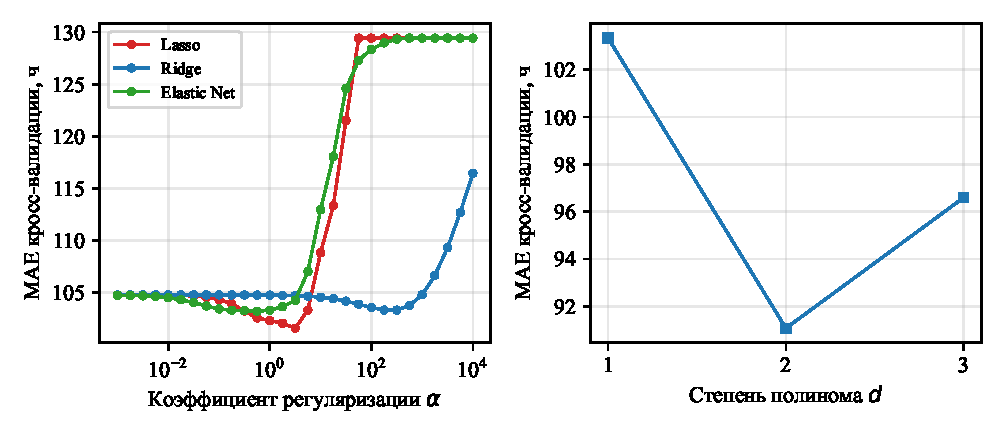
\includegraphics[width=\textwidth]{figures/fig3_validation.pdf}
\caption{MAE кросс-валидации в зависимости от коэффициента регуляризации
(слева) и степени полинома (справа), конфигурация Б}
\label{fig:validation}
\end{figure}

На этих же кривых видны классические признаки переобучения и недообучения.
При сильной регуляризации (правый край левой панели) MAE КВ растёт у всех
моделей~--- модель зажата и недообучается. Без регуляризации картина
обратная: наивный МНК достигает на обучении $R^2=\OlsRtwoTrain$, но его
MAE КВ (\OlsMAECV~ч) в несколько раз хуже~--- модель подогналась под
обучающие записи и не держит проверку. Полином третьей степени в
конфигурации Б не улучшает MAE КВ по сравнению со второй, хотя обучающая
ошибка при расширении признаков падает,~--- это признак того, что
дополнительная сложность начинает подгонять шум; поэтому третья степень
в выборе итоговой модели не участвует.

Первый результат работы получился отрицательным, и он оказался самым
поучительным. Наивная МНК на сырой цели \eqref{eq:rul} на отложенном
испытании достигает MAE \OlsMAETest~ч при минимальном прогнозе
\OlsMinPred~ч: обученная экстраполировать линейный тренд ресурса, модель
прогнозирует отрицательное «время до конца»~--- операцию, которая по смыслу
уже состоялась. При этом в кросс-валидации тот же МНК выглядит пристойно
(MAE \OlsMAECV~ч). Интерполяционная оценка полностью маскирует катастрофу
переноса~--- цель вида \eqref{eq:rul} в принципе не пригодна для линейной
экстраполяции, и никакая регуляризация этого не исправит.

После введения цели \eqref{eq:cap} и ограничения признаков диапазоном
обучения MAE КВ лучших моделей снижается в несколько раз
(табл.~\ref{tab:hyper}). По правилу 1SE (порог \BestThrOneSE~ч) среди
кандидатов минимальное эффективное число параметров имеет лассо-регрессия
конфигурации Б: \BestHyper, \BestDof{} параметров при \BestNFeat{} признаках.
Она и выбрана итоговой. Отметим, что в кандидаты попали и модели
конфигурации А с лучшим MAE КВ~--- правило 1SE предпочло им разреженную
модель по худшему подшипнику; как покажет следующий раздел, это оказалось
счастливым выбором.

\subsection{Окончательная модель и интерпретация}

Метрики итоговой модели: на обучении MAE \BestMAETrain~ч, в кросс-валидации
MAE $\BestMAECV \pm \BestMAECVstd$~ч, на отложенном испытании MAE
\BestMAETest~ч, RMSE \BestRMSETest~ч, $R^2 = \BestRtwoTest$, ранговая
корреляция Спирмена $\rho = \BestRhoTest$ (табл.~\ref{tab:test}).
Низкое $R^2$ на обучении~--- ожидаемое следствие усечённой цели: на плато
исправного состояния \eqref{eq:cap} модель закономерно не различает записи
с $RUL$ от $C$ до максимума.

Бутстрэп-интервалы коэффициентов (таблица~\ref{tab:coef},
рисунок~\ref{fig:bootstrap}) показывают, что знаки и порядок ключевых
коэффициентов устойчивы. Лассо оставило пять ненулевых признаков из девяти,
и среди них три доминируют: \texttt{max\_e1\_2khz}, \texttt{max\_varlogrel}
и \texttt{max\_crestlogrel}~--- спектральная доля полосы 1--2~кГц и
нормированные дисперсия с пик-фактором худшего подшипника. Все три
коэффициента отрицательны: рост амплитудных и среднечастотных характеристик
сокращает прогноз ресурса, ровно как предполагалось в гипотезах H1 и H2.
Обнулённые лассо признаки (RMS, эксцесс) дублировали уже учтённую
информацию~--- они сильно коррелируют с оставшимися амплитудными
характеристиками, и лассо оставило по одному представителю каждой группы
коррелированных признаков; чувствительность к коррелированности проявилась
именно в отборе, а не в нестабильности знаков: бутстрэп-медианы оставшихся
коэффициентов уверенно не проходят через нуль. Полезно, что модель
избавилась от дублирующих признаков сама.

\begin{table}[H]
\centering
\caption{Бутстрэп-оценки ненулевых коэффициентов итоговой модели (95\,\%-ные доверительные интервалы)}\label{tab:coef}
\begin{tabular}{p{5.6cm}rrrr}
\toprule
Признак & Медиана & 2,5\,\% & 97,5\,\% & Доля $\beta>0$ \\
\midrule
max\_e1\_2khz & \textminus{}39,963 & \textminus{}43,532 & \textminus{}36,588 & 0,00 \\
max\_varlogrel & \textminus{}28,153 & \textminus{}31,652 & \textminus{}24,578 & 0,00 \\
max\_crestlogrel & \textminus{}3,310 & \textminus{}5,545 & \textminus{}1,058 & 0,00 \\
max\_e0\_1khz & 2,573 & 0,000 & 4,614 & 0,97 \\
max\_e5\_10khz & \textminus{}1,277 & \textminus{}4,779 & 0,000 & 0,00 \\
\bottomrule
\end{tabular}
\end{table}

\begin{figure}[H]
\centering
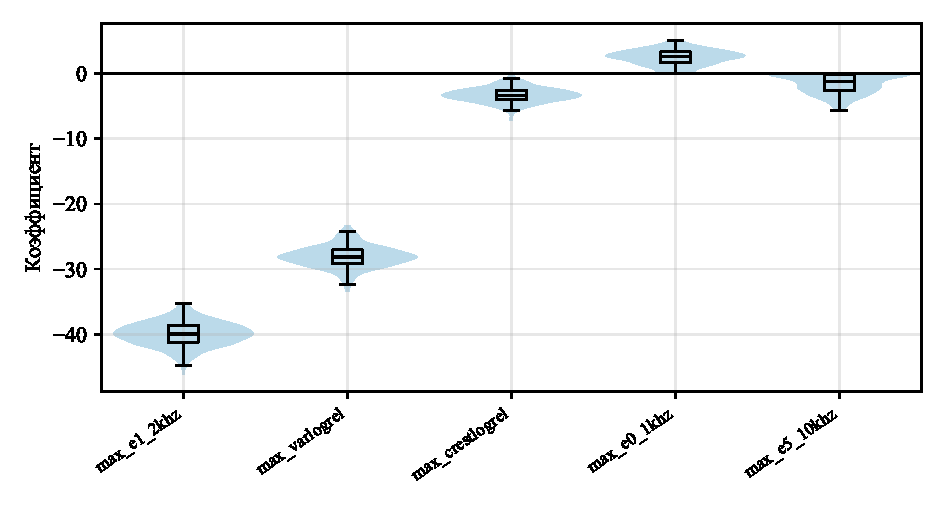
\includegraphics[width=0.9\textwidth]{figures/fig6_bootstrap.pdf}
\caption{Бутстрэп-распределения коэффициентов итоговой модели
(топ-8 по модулю медианы)}
\label{fig:bootstrap}
\end{figure}

\subsection{Диагностика остатков}

Остатки отложенного испытания (рисунок~\ref{fig:residuals}) не показывают
грубой систематической зависимости от прогноза: корреляция остатков
с прогнозом $\rho$ = \RhoResidPred{} (таблица~\ref{tab:resid}). Основной
источник разброса~--- ранний участок испытания 2, где деградация ещё не
проявилась в амплитуде, а прогноз уже снижен усечённой целью; корреляция
остатков с нормированной амплитудой худшего подшипника ($\rho$ = \RhoResidRMS)
умеренная, знаковая систематика отсутствует. Зависимость от эксцесса слабая
($\rho$ = \RhoResidKurt).

\begin{figure}[H]
\centering
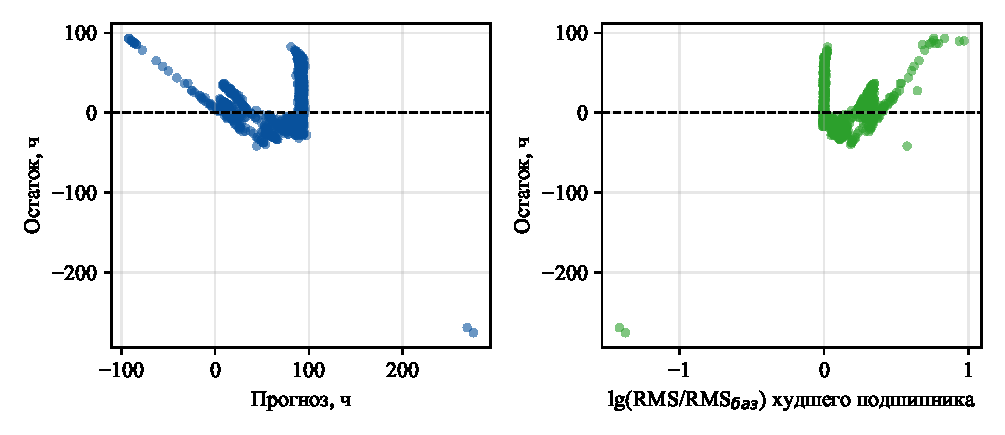
\includegraphics[width=\textwidth]{figures/fig5_residuals.pdf}
\caption{Остатки итоговой модели на отложенном испытании: против прогноза
(слева) и против нормированной амплитуды худшего подшипника (справа)}
\label{fig:residuals}
\end{figure}

\begin{table}[H]
\centering
\caption{Ранговые корреляции остатков отложенного испытания с факторами}\label{tab:resid}
\begin{tabular}{p{8.5cm}c}
\toprule
Фактор & Коэффициент Спирмена \\
\midrule
Прогноз модели & 0,29 \\
lg(RMS/RMS$_{\text{баз}}$) худшего подшипника & \textminus{}0,31 \\
Эксцесс худшего подшипника & 0,11 \\
\bottomrule
\end{tabular}
\end{table}

% ============================================================================
\section{ОБСУЖДЕНИЕ: ПЕРЕНОС НА ОТЛОЖЕННОЕ ИСПЫТАНИЕ}

\subsection{Качество переноса}

Сопоставление измеренного и предсказанного ресурса приведено на
рисунке~\ref{fig:predactual}, сравнение интерполяционной и переносной
оценок~--- на рисунке~\ref{fig:transfer} и в таблице~\ref{tab:test}.

\begin{figure}[H]
\centering
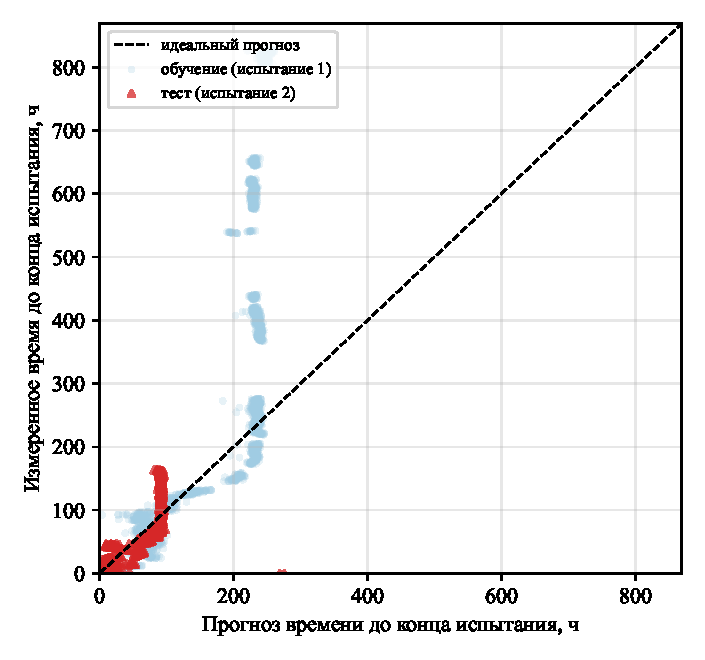
\includegraphics[width=0.66\textwidth]{figures/fig4_pred_actual.pdf}
\caption{Измеренное и предсказанное время до конца испытания}
\label{fig:predactual}
\end{figure}

\begin{figure}[H]
\centering
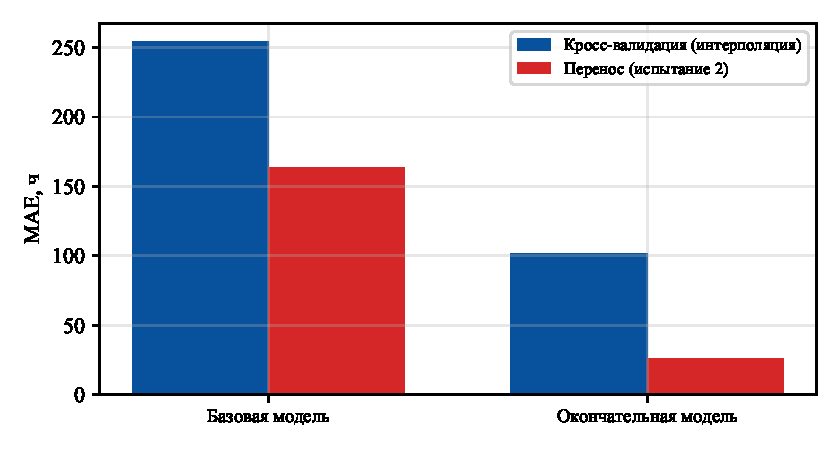
\includegraphics[width=0.8\textwidth]{figures/fig7_transfer.pdf}
\caption{MAE кросс-валидации (интерполяция) и отложенного испытания (перенос)}
\label{fig:transfer}
\end{figure}

\begin{table}[H]
\centering
\caption{Качество прогнозов на отложенном испытании}\label{tab:test}
\begin{tabular}{p{3.4cm}c ccc}
\toprule
Модель & Призн. & $R^2$ (тест) & MAE (тест), ч & $\rho$ Спирмена \\
\midrule
Базовая (медиана) & А & \textminus{}11,93 & 163,5 & --- \\
МНК (наивная) & А & \textminus{}14122,62 & 3648,1 & \textminus{}0,41 \\
МНК + цель min(RUL, C) & А & \textminus{}1441,21 & 1724,2 & \textminus{}0,31 \\
Полином + гребень & А & \textminus{}7,14 & 80,8 & \textminus{}0,57 \\
Ridge & А & \textminus{}7,14 & 80,8 & \textminus{}0,57 \\
Lasso & А & \textminus{}18,01 & 164,0 & \textminus{}0,48 \\
Elastic Net & А & \textminus{}7,09 & 81,2 & \textminus{}0,58 \\
МНК (наивная) & Б & \textminus{}464,75 & 996,4 & 0,57 \\
МНК + цель min(RUL, C) & Б & \textminus{}1,48 & 65,0 & 0,69 \\
Полином + гребень & Б & \textminus{}98,51 & 448,4 & \textminus{}0,79 \\
Ridge & Б & \textminus{}0,17 & 40,9 & 0,79 \\
Lasso & Б & 0,47 & 25,9 & 0,78 \\
Elastic Net & Б & 0,15 & 32,7 & 0,79 \\
\bottomrule
\end{tabular}
\end{table}

Здесь и находится главный вывод работы. Модели конфигурации А «по
подшипникам» обучаются на отказах подшипников №3 и №4 и в кросс-валидации
показывают лучший MAE~--- тем обиднее (и тем показательнее) то, что
происходит на тесте. Когда отказал подшипник №1, каналы, на которые эти
модели оперлись при обучении, оказались здоровыми: модели конфигурации А
переносятся плохо, у части из них $R^2$ уходит в глубокий минус, а ранговая
корреляция становится отрицательной~--- модель упорядочивает записи
наоборот (табл.~\ref{tab:test}). Агрегат «худший подшипник» (конфигурация Б)
по построению не зависит от номера отказавшего узла и переносится
существенно лучше: лассо~--- MAE \BestMAETest~ч, упругая сеть~---
\ENetBMAETest~ч, Ridge~--- \RidgeBMAETest~ч против \BaseMAETest~ч у базовой
модели. Гипотеза H3 подтвердилась.

Отдельная история~--- полином. Вторая степень улучшила MAE КВ конфигурации Б
(91~ч против 103~ч у линейного Ridge, табл.~\ref{tab:hyper}), то есть
формально дала то самое «подтверждённое КВ улучшение». Но на отложенном
испытании полиномиальная модель деградирует катастрофически
(MAE \RidgePolyBMAETest~ч): у границ диапазона обучения квадратичные и
кубические комбинации признаков порождают неустойчивые прогнозы, и ограничение
признаков, которое спасает линейную модель, от комбинаций уже не защищает.
Полиномиальные признаки улучшили интерполяцию и разрушили перенос, поэтому
в итоговой модели от них отказано в пользу чистой линейности. Третья степень
в правилах выбора участвовать не смогла: её лучшие MAE КВ не превзошли
вторую.

\subsection{Интерполяция против переноса}

Для итоговой модели кросс-валидация даёт MAE \BestMAECV~ч, а отложенное
испытание~--- \BestMAETest~ч: перенос оказался заметно лучше
интерполяционной оценки. Причина в устройстве складок КВ: внутри
обучающего испытания, которое длится \DurTrain~ч, складки включают участки
с медленно меняющейся усечённой целью, и задача в КВ объективно тяжелее,
чем на коротком (\DurHoldout~ч) испытании 2. Для конфигурации А соотношение
обратное: MAE КВ у неё лучше, а тест хуже. Это значит, что совпадение или
расхождение интерполяционной и переносной оценок не гарантировано ни в какую
сторону: кросс-валидация в принципе не может предсказать качество переноса
при смене отказавшего компонента, потому что такого сценария нет в
обучающих данных.

Практический вывод из этого такой. При проектировании моделей мониторинга
агрегатов стоит заранее закладывать отказ в любой компонент: агрегация по
худшему элементу, нормированные и безразмерные признаки, ограничение
экстраполяции и разреженные модели. Оптимизация чисто интерполяционного
качества на конкретном испытании может улучшать числа в отчёте, одновременно
ухудшая поведение модели в реальном применении.

% ============================================================================
\struct{ЗАКЛЮЧЕНИЕ}

В работе выполнено задание 1 (вариант 13): по стендовым испытаниям NASA IMS
построены линейные модели прогноза времени, остающегося до конца испытания.
Основные результаты:

\begin{enumerate}
  \item Из сигналов извлечены физически мотивированные признаки: RMS,
  дисперсия, эксцесс, пик-фактор и доли энергии в пяти широких полосах,
  с нормировкой амплитудных признаков на здоровый базовый уровень
  (\ref{eq:logrel}). Рассмотрены две конфигурации признаков: «по
  подшипникам» (36 признаков) и «худший подшипник» (9 признаков).
  \item Показана несостоятельность наивной постановки: МНК на сырой цели
  \eqref{eq:rul} даёт на отложенном испытании MAE \OlsMAETest~ч с
  отрицательными прогнозами до \OlsMinPred~ч, оставаясь приемлемым
  в кросс-валидации. Физически мотивированная постановка с целью
  $\min(RUL, C)$ и ограничение признаков диапазоном обучения устраняют
  проблему.
  \item Гиперпараметры (порог $C$, коэффициент регуляризации $\alpha$,
  соотношение $l_1$, степень полинома) подобраны только по обучающему
  испытанию скользящей кросс-валидацией по временным складкам; отложенное
  испытание использовано однократно.
  \item По правилу одного стандартного отклонения выбрана лассо-регрессия
  по признакам худшего подшипника (\BestHyper; \BestDof{} параметров).
  На отложенном испытании: MAE \BestMAETest~ч, RMSE
  \BestRMSETest~ч, $R^2=\BestRtwoTest$, $\rho=\BestRhoTest$ против
  \BaseMAETest~ч у базовой модели.
  \item Бутстрэп подтвердил устойчивость знаков ключевых коэффициентов;
  диагностика остатков не выявила грубой систематики.
  \item Установлено, что интерполяционная (кросс-валидационная) оценка
  не гарантирует переноса: модели по отдельным подшипникам выигрывают
  в КВ, но терпят неудачу на отложенном испытании, а полиномиальные
  признаки разрушают перенос; устойчивый перенос дают агрегация
  по худшему элементу и разреженные модели.
\end{enumerate}

Все числа отчёта генерируются программно; отчёт собирается одной
командой \texttt{python build.py}.

% ============================================================================
\struct{СПИСОК ИСПОЛЬЗОВАННЫХ ИСТОЧНИКОВ}

{\sloppy
\begin{thebibliography}{9}
\bibitem{qiu2006} Qiu, H. Wavelet filter-based weak signature detection method
and its application on rolling element bearing prognostics / H. Qiu, J. Lee,
J. Lin, G. Yu // Journal of Sound and Vibration.~--- 2006.~--- Vol. 289,
No. 4--5.~--- P. 1066--1090.
\bibitem{ims} Bearing Data Set~// NASA Ames Prognostics Data Repository:
[сайт].~--- URL: https://www.nasa.gov/intelligent-systems-division/
discovery-and-systems-health/pcoe/pcoe-data-set-repository/ (дата обращения:
13.11.2026).~--- Текст: электронный.
\bibitem{assignment} Задания по дисциплине «Машинное обучение»~// [сайт].~---
URL: https://ckpeiika.github.io/pages/ml-assignments.html (дата обращения:
13.11.2026).~--- Текст: электронный.
\bibitem{sklearn} Pedregosa, F. Scikit-learn: Machine Learning in Python /
F. Pedregosa [et al.] // Journal of Machine Learning Research.~--- 2011.~---
Vol. 12.~--- P. 2825--2830.
\bibitem{hastie} Hastie, T. The Elements of Statistical Learning: Data Mining,
Inference, and Prediction / T. Hastie, R. Tibshirani, J. Friedman.~---
2nd ed.~--- New York : Springer, 2009.~--- 745 p.
\bibitem{tibshirani} Tibshirani, R. Regression Shrinkage and Selection via
the Lasso / R. Tibshirani // Journal of the Royal Statistical Society,
Series B.~--- 1996.~--- Vol. 58, No. 1.~--- P. 267--288.
\bibitem{zou2005} Zou, H. Regularization and variable selection via the
elastic net / H. Zou, T. Hastie // Journal of the Royal Statistical Society,
Series B.~--- 2005.~--- Vol. 67, No. 2.~--- P. 301--320.
\bibitem{randall} Randall, R. B. Vibration-based Condition Monitoring:
Industrial, Aerospace and Automotive Applications / R. B. Randall.~---
Chichester : Wiley, 2011.~--- 320 p.
\bibitem{efron} Efron, B. An Introduction to the Bootstrap / B. Efron,
R. J. Tibshirani.~--- New York : Chapman \& Hall/CRC, 1993.~--- 436 p.
\end{thebibliography}
}

% ============================================================================
% Приложения
% ============================================================================
\clearpage
\setcounter{figure}{0}
\renewcommand{\thefigure}{А.\arabic{figure}}

\begin{center}\bfseries ПРИЛОЖЕНИЕ А\end{center}
\begin{center}Динамика эксцесса по подшипникам\end{center}
\addcontentsline{toc}{section}{ПРИЛОЖЕНИЕ А. Динамика эксцесса по подшипникам}

\begin{figure}[H]
\centering
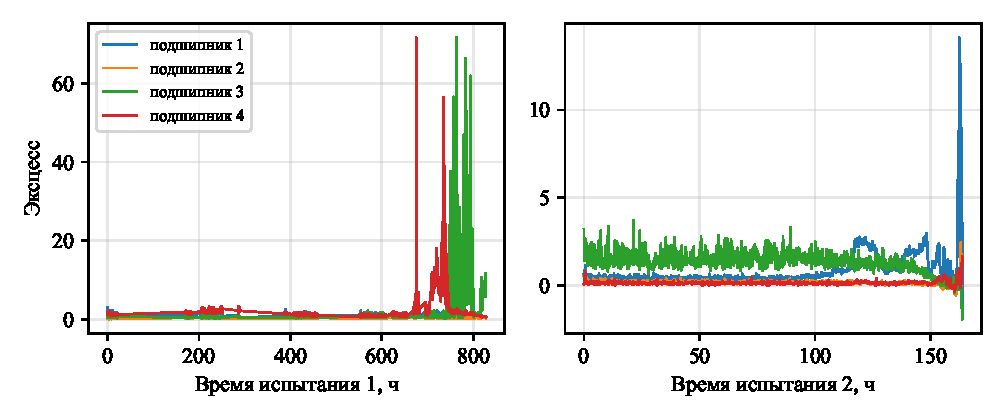
\includegraphics[width=\textwidth]{figures/figD1_kurtosis.pdf}
\caption{Эксцесс сигналов по подшипникам в течение испытаний}
\end{figure}

\clearpage
\begin{center}\bfseries ПРИЛОЖЕНИЕ Б\end{center}
\begin{center}Состав признаков\end{center}
\addcontentsline{toc}{section}{ПРИЛОЖЕНИЕ Б. Состав признаков}

\begin{sloppypar}
\noindent Конфигурация А «по подшипникам»~--- для каждого подшипника
$b \in \{1,2,3,4\}$ вычисляются девять признаков (36 всего):

\begin{itemize}
  \item \texttt{b\_rms\_logrel}~--- $\lg(\mathrm{RMS}/\mathrm{RMS}_{\text{баз}})$;
  \item \texttt{b\_var\_logrel}~--- $\lg(\sigma^2/\sigma^2_{\text{баз}})$;
  \item \texttt{b\_crest\_logrel}~--- $\lg(c_{\text{peak}}/c_{\text{peak,баз}})$;
  \item \texttt{b\_kurt}~--- эксцесс;
  \item \texttt{b\_e0\_1khz}~\ldots~\texttt{b\_e5\_10khz}~--- доли энергии в полосах
  0--1, 1--2, 2--3, 3--5, 5--10~кГц.
\end{itemize}

\noindent Конфигурация Б «худший подшипник»~--- по каждому из девяти признаков
берётся поэлементный максимум по четырём подшипникам, признак получает имя
\texttt{max\_rms\_logrel}, \texttt{max\_var\_logrel}, \texttt{max\_crest\_logrel},
\texttt{max\_kurt}, \texttt{max\_e0\_1khz}~\ldots~\texttt{max\_e5\_10khz},
всего 9 признаков. Базовый уровень признака~--- медиана значений первых 10\,\%
записей соответствующего испытания.
\end{sloppypar}

\end{document}
